\section{Projeto Base e Resultados}\label{sec:projeto-base}
O News Architecture Demo implementa 12 notícias fictícias, detalhes e
favoritos. Usa Kotlin, Compose/Material 3, ViewModels, Flow, Room, Hilt e
Gradle Kotlin DSL. O catálogo é imutável e empacotado; Room persiste apenas
IDs favoritos. A demonstração funciona sem rede, mas não implementa a
sincronização do original.

Os quatro módulos são \texttt{app}, \texttt{core},
\texttt{feature:\allowbreak news} e \texttt{feature:\allowbreak favorites}
(Figura~\ref{fig:demo}). O núcleo separa modelos, domínio, dados, persistência
e UI em pacotes. Banco, entidade e DAO são internos ao módulo. As features
não dependem entre si, e o aplicativo coordena a navegação por callbacks.

\texttt{Observe\allowbreak News\allowbreak With\allowbreak Favorites\allowbreak Use\allowbreak Case} combina catálogo e favoritos e
ordena por data, sendo reutilizado pelos três ViewModels. O colaborador
\texttt{Feed\allowbreak State\allowbreak Holder} compartilha comportamento de apresentação por
composição: observação, estados, mensagens e gravações pendentes. As telas
não acessam DAOs. Salvar/remover é idempotente; durante a escrita, o marcador
fica desabilitado. Uma falha mantém o conteúdo e oferece nova tentativa.

\begin{figure*}[t]
\centering
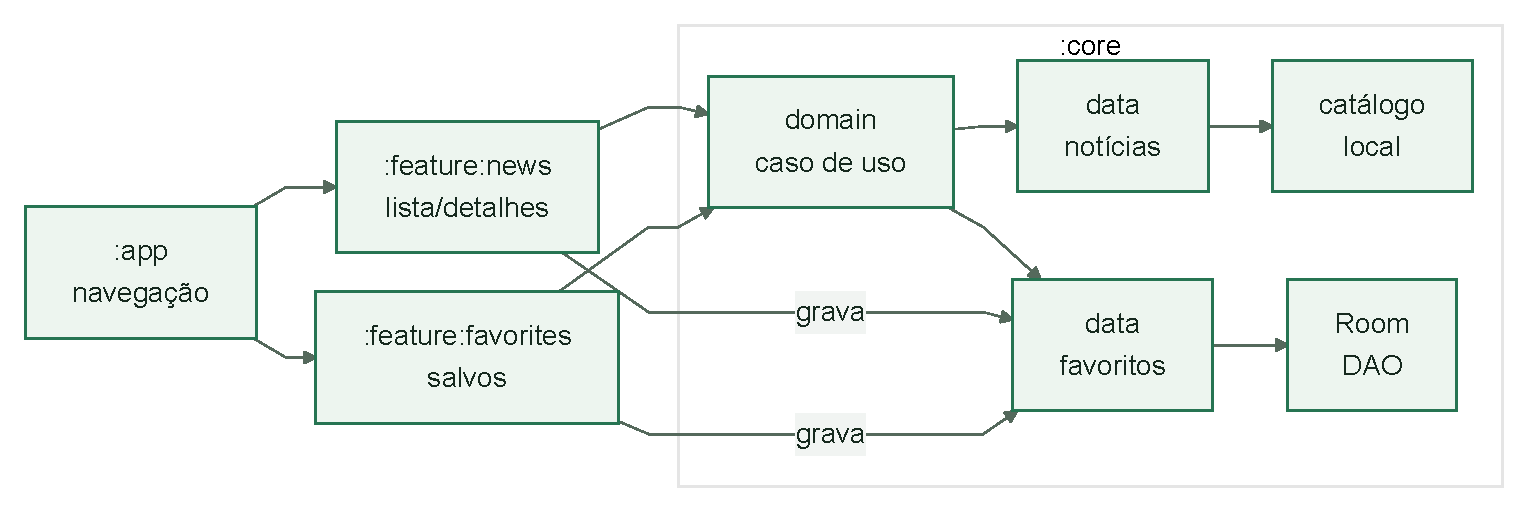
\includegraphics[width=\textwidth]{imagens/05-demo.pdf}
\caption{Arquitetura implementada na demonstração. Setas indicam dependências
ou chamadas; a atualização observável percorre o caminho inverso até a UI.}
\Description{O aplicativo coordena duas features. Ambas usam um caso de uso no núcleo e gravam pelo repositório de favoritos. O domínio combina catálogo local e favoritos Room.}
\label{fig:demo}
\end{figure*}

A validação aprovou \UnitTests{} testes unitários e \InstrumentedTests{}
instrumentados: caso de uso, repositórios, três ViewModels, Room real,
reabertura de arquivo e navegação Compose. O roteiro no emulador também
confirmou o favorito após encerrar e reabrir o processo. O lint não apontou
erros; avisos sobre versões mais novas foram preservados, pois as versões
foram fixadas por compatibilidade.

As verificações encontraram zero ciclos, zero dependências entre features e
zero referências proibidas à persistência no recorte da UI. Cinco classes
foram testadas com fakes; a chamada unitária levou \UnitSeconds{} s, com
cache e daemon ativos. Os cinco controles amostrados atenderam às verificações
de rótulo e área mínima de 48 dp.

No APK debug, em emulador Android 16 ARM64, dez reinícios do processo
apresentaram mediana de \StartupMedian{} ms
(intervalo \StartupMin{}--\StartupMax{} ms) para \texttt{Total\allowbreak Time}.
Dez gravações com Room em memória tiveram latência mediana de \FavoriteMedian{}
ms até a emissão combinada. Uma amostra após o roteiro registrou
\MemoryPss{} MiB de PSS. Essas observações não medem desempenho do NiA,
latência final de renderização ou comportamento em aparelhos físicos.
